\documentclass{standalone}
\usepackage{tikz}

\begin{document}

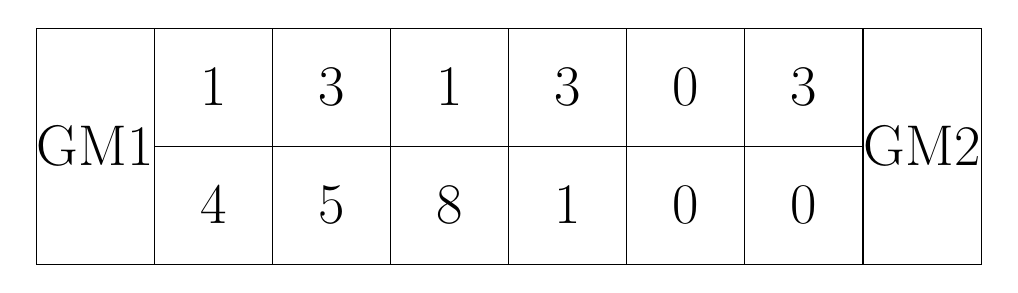
\begin{tikzpicture}[scale=1.5, font=\huge]
% Cases
\foreach \x/\stones in {0/4,1/5,2/8,3/1,4/0,5/0} {
  \draw (\x,0) rectangle ++(1,1) node[pos=.5] {\stones};
}
\foreach \x/\stones in {0/1,1/3,2/1,3/3,4/0,5/3} {
  \draw (\x,1) rectangle ++(1,1) node[pos=.5] {\stones};
}
% Grands magasins
\draw (-1,0) rectangle ++(1,2) node[midway] {GM1};
\draw (6,0) rectangle ++(1,2) node[midway] {GM2};
% Labels
%\foreach \x in {1,2,...,6} {
%  \draw (\x-0.5,1.5) node {$C_\x$};
%}
%\foreach \x in {1,2,...,6} {
%  \draw (\x-0.5,0.5) node {$C_\x$};
%}

\end{tikzpicture}

\end{document}
